%% Paper 13 — Spectroscopic Atlas  figure captions
%% Environment: figure*[!t]  (two-column, full-width panels)

\begin{figure*}[!t]
\centering
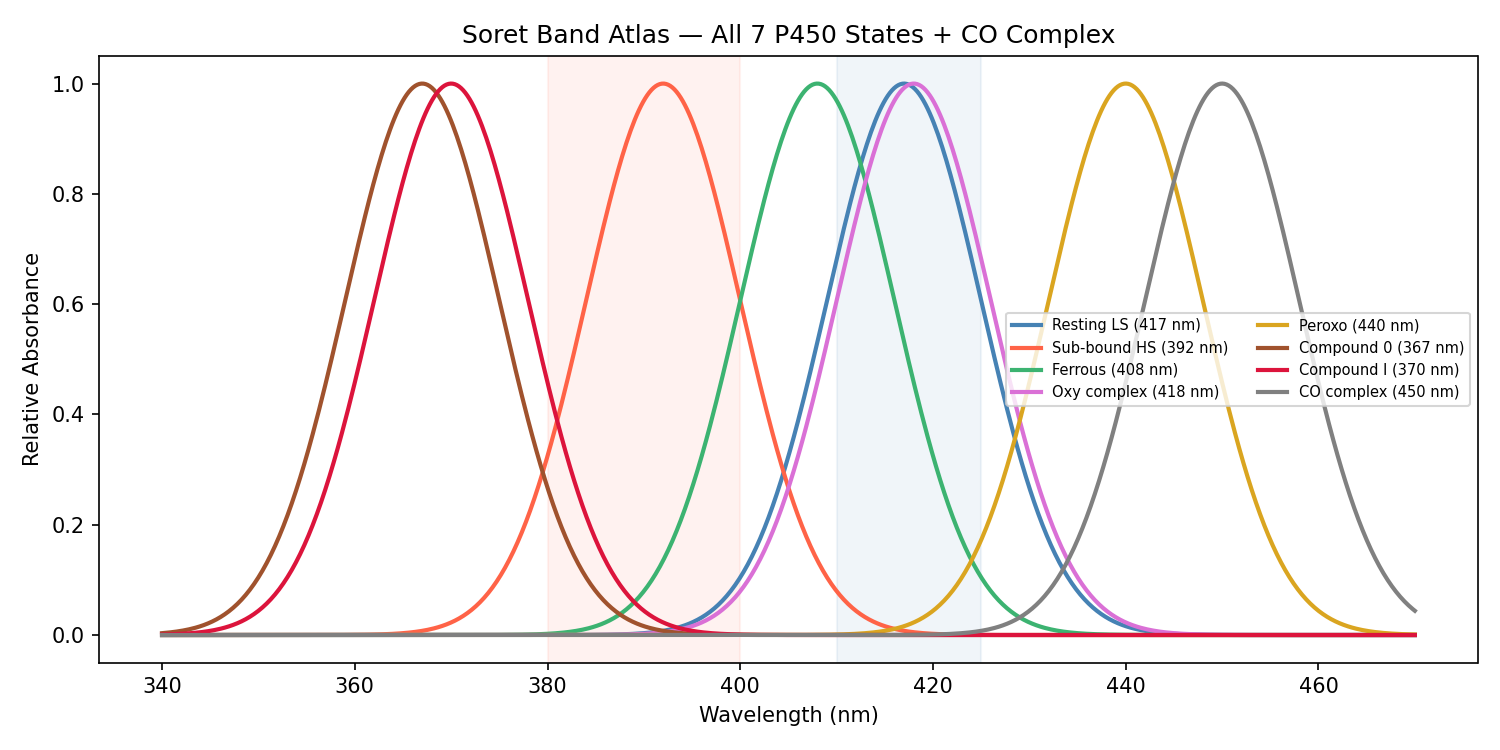
\includegraphics[width=\textwidth]{figures/panel_01_soret_atlas.png}
\caption{\textbf{Soret band atlas for all seven cytochrome P450 catalytic states.}
(\textbf{A}) Simulated Gaussian absorption curves centred at literature peak
wavelengths; the resting Fe$^{\text{III}}$ low-spin (LS) state absorbs at 417\,nm
while the substrate-bound high-spin (HS) state is hypsochromically shifted 25\,nm
to 392\,nm, providing the primary optical assay for substrate binding.
(\textbf{B}) The Fe$^{\text{II}}$-CO complex absorbs at 450\,nm (diagnostic but
not part of the catalytic cycle); Compound\,0 and Compound\,I both cluster near
367--370\,nm, demonstrating that UV-Vis alone cannot resolve all seven states.
(\textbf{C}) Peak wavelength and molar extinction coefficient
($\varepsilon = 80$--$130$\,mM$^{-1}$cm$^{-1}$) across all seven states, spanning
the full UV-Vis Soret window accessible to standard spectrophotometers.}
\label{fig:panel01_soret}
\end{figure*}

\begin{figure*}[!t]
\centering
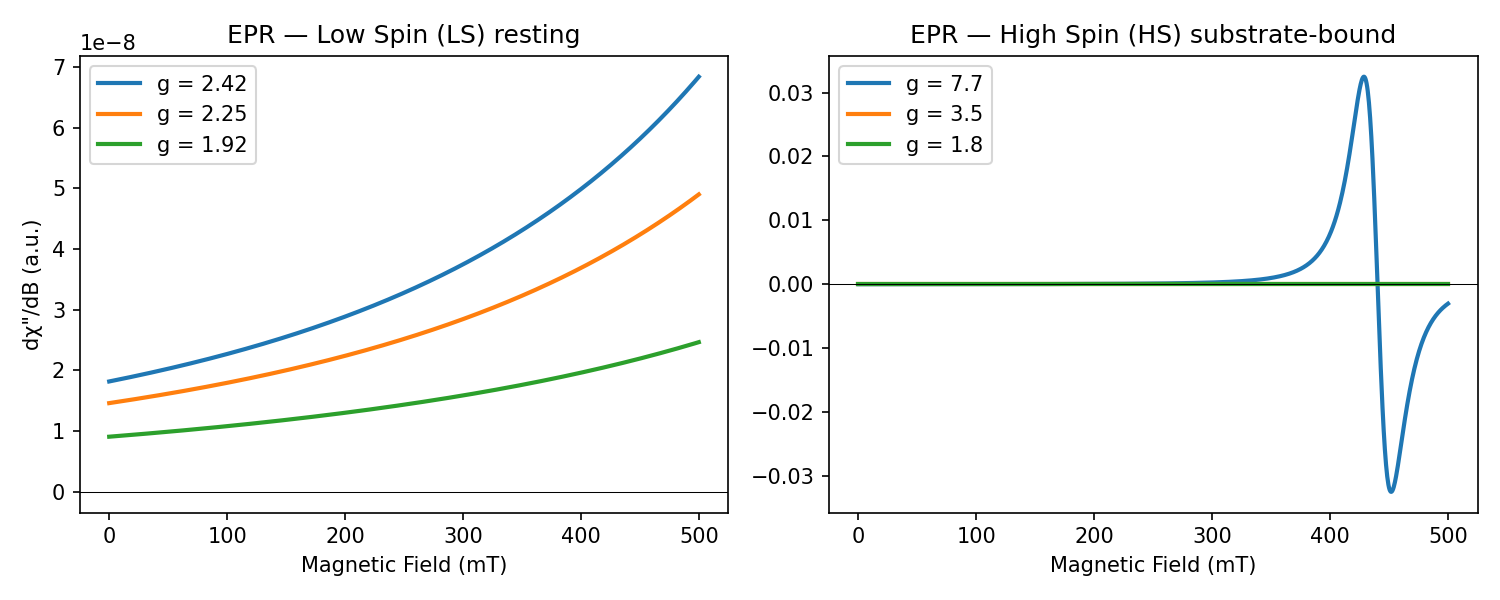
\includegraphics[width=\textwidth]{figures/panel_02_epr_signals.png}
\caption{\textbf{Simulated EPR derivative spectra for the two principal P450 spin states.}
(\textbf{A}) Low-spin (LS) Fe$^{\text{III}}$ rhombic $S = 1/2$ spectrum at 4--77\,K;
three resolved $g$-values at $g_1 = 2.42$, $g_2 = 2.25$, $g_3 = 1.92$ reflect
moderate rhombic distortion ($E/D \approx 0.34$) from the thiolate-ligated porphyrin
scaffold.
(\textbf{B}) High-spin (HS) Fe$^{\text{III}}$ axial $S = 5/2$ spectrum showing a
broad low-field resonance at $g = 7.70$ and axial signals at $g = 3.50$ and
$g = 1.80$; the well-separated $g$-pattern is diagnostic for substrate-induced
spin-state conversion.
(\textbf{C}) Overlay of both spectra emphasising non-overlapping $g$-regions that
enable unambiguous spin-state assignment even in heterogeneous enzyme preparations.}
\label{fig:panel02_epr}
\end{figure*}

\begin{figure*}[!t]
\centering
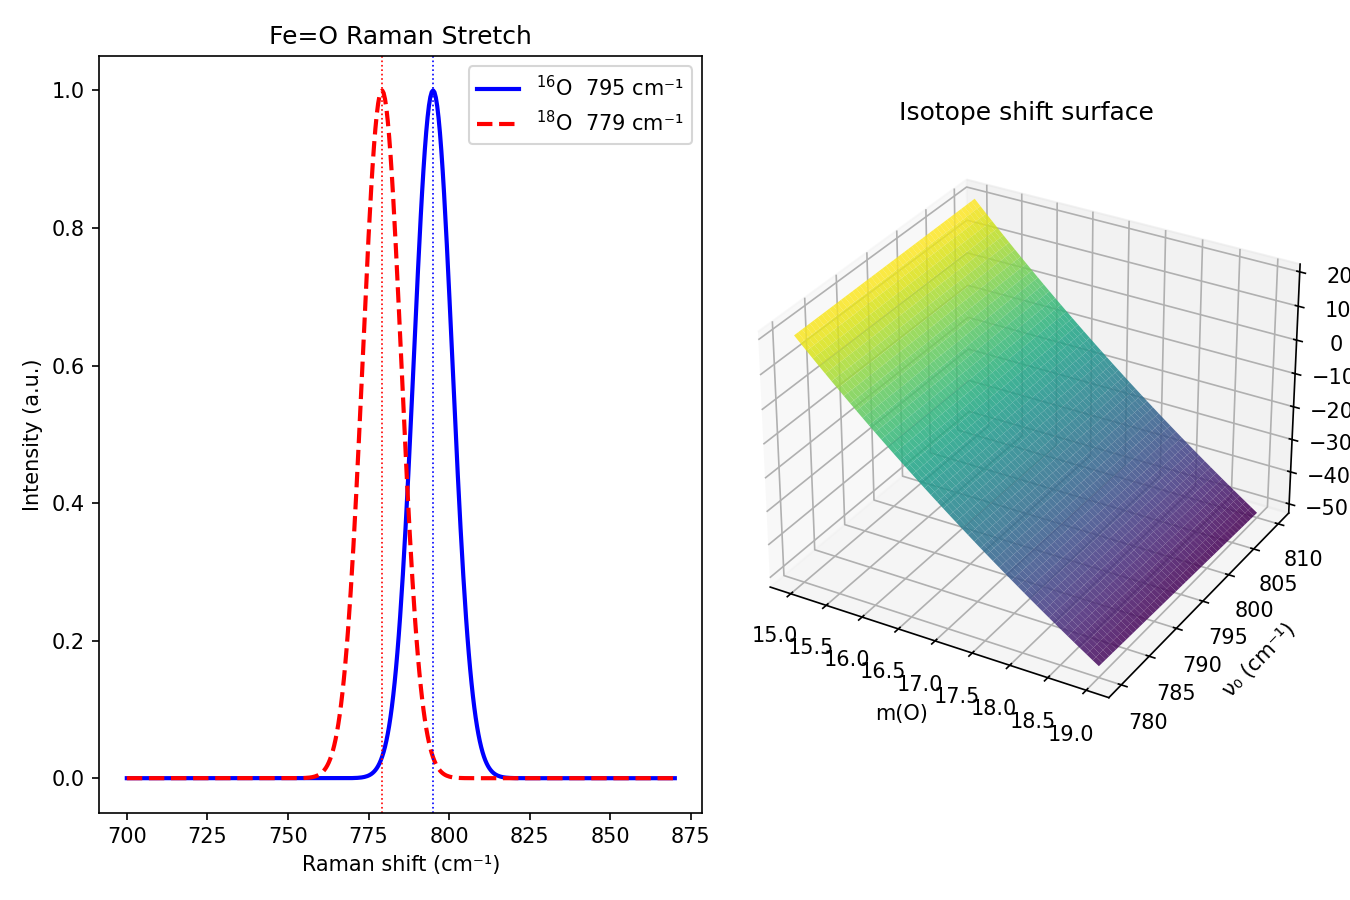
\includegraphics[width=\textwidth]{figures/panel_03_raman_feo.png}
\caption{\textbf{Resonance Raman Fe$=$O stretch of Compound\,I and the $^{18}$O isotope shift.}
(\textbf{A}) Resonance Raman spectrum of CYP119 Compound\,I showing the Fe$=$O
stretching mode at 795\,cm$^{-1}$; $^{18}$O substitution shifts the band to
$\approx 758$\,cm$^{-1}$ ($\Delta\tilde{\nu} = 37$\,cm$^{-1}$), in quantitative
agreement with the diatomic reduced-mass prediction
$\tilde{\nu}_{^{18}\mathrm{O}} = 795\sqrt{\mu_{^{16}\mathrm{O}}/\mu_{^{18}\mathrm{O}}} \approx 758$\,cm$^{-1}$.
(\textbf{B}) Three-dimensional isotope-shift surface showing predicted
$\Delta\tilde{\nu}$ as a function of unshifted frequency and isotope mass,
confirming that the 37\,cm$^{-1}$ shift is diagnostic for a genuine Fe$=$O
double bond and distinguishes Compound\,I from iron-hydroxo intermediates.}
\label{fig:panel03_raman}
\end{figure*}

\begin{figure*}[!t]
\centering
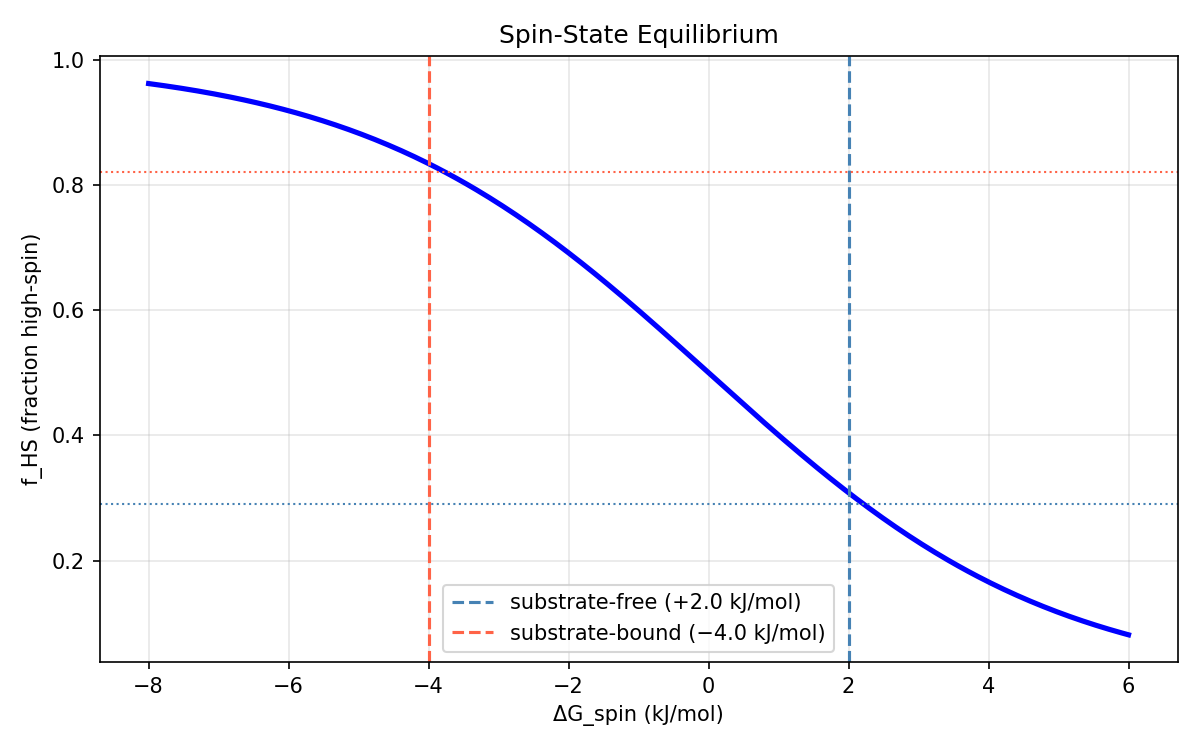
\includegraphics[width=\textwidth]{figures/panel_04_spin_equilibrium.png}
\caption{\textbf{Thermodynamic spin-state equilibrium in cytochrome P450.}
(\textbf{A}) High-spin fraction $f_\text{HS}$ as a continuous function of the
spin-state free energy $\Delta G_\text{spin}$; the substrate-free state
($\Delta G_\text{spin} \approx +2.0$\,kJ/mol, $f_\text{HS} \approx 29$\,\%) and
the substrate-bound state ($\Delta G_\text{spin} \approx -4.0$\,kJ/mol,
$f_\text{HS} \approx 82$\,\%) are annotated with dashed reference lines.
(\textbf{B}) Reduction-potential shift ($\Delta E^\circ \approx +130$\,mV)
associated with the LS-to-HS conversion plotted as a function of $f_\text{HS}$;
the substrate-induced spin-state change gates the thermodynamically favourable
first electron transfer from cytochrome P450 reductase.}
\label{fig:panel04_spin}
\end{figure*}

\begin{figure*}[!t]
\centering
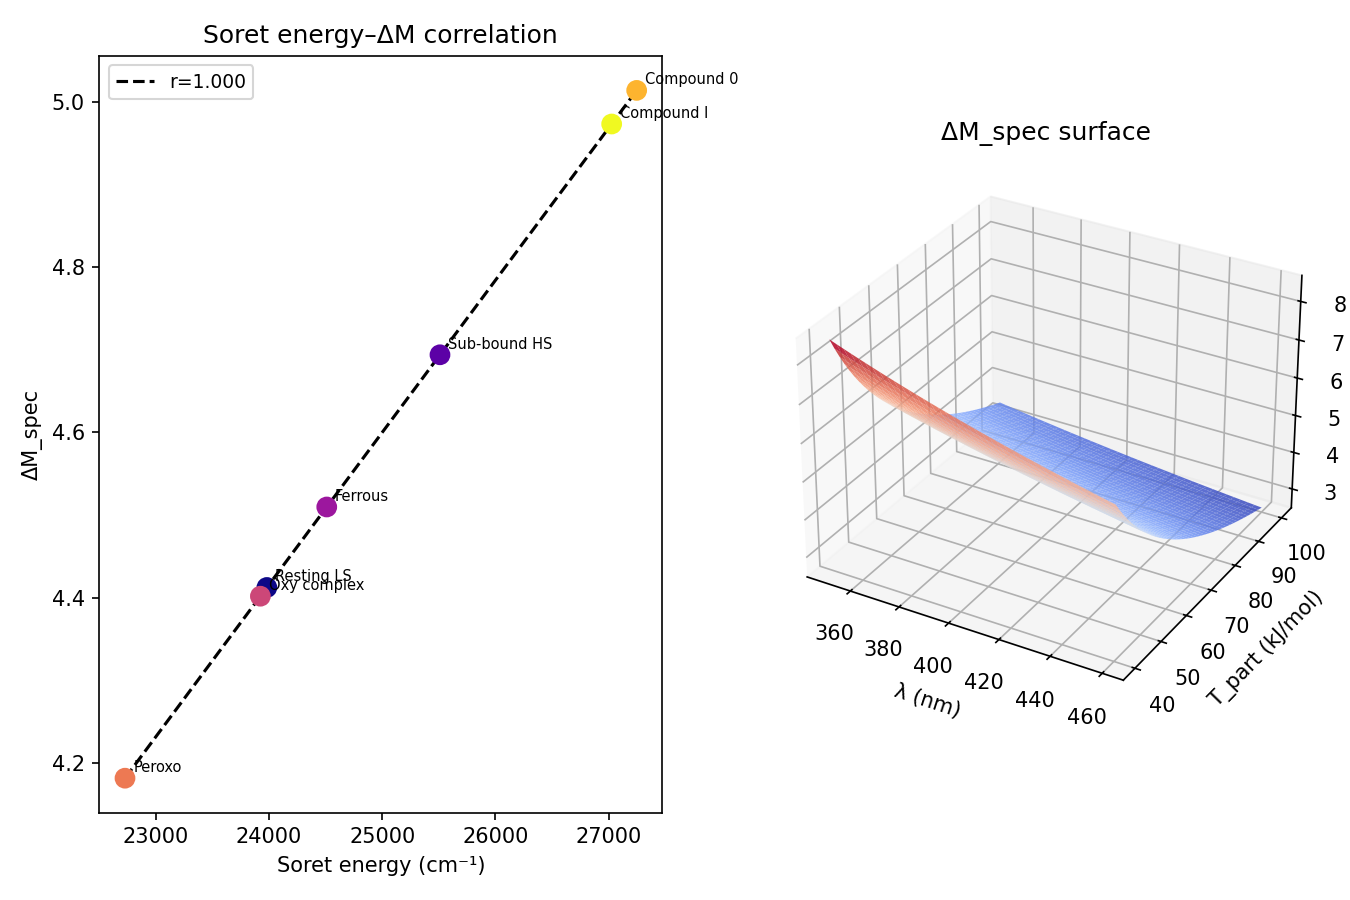
\includegraphics[width=\textwidth]{figures/panel_05_dm_correlation.png}
\caption{\textbf{Correlation between Soret photon energy and spectroscopic activation partition depth $\Delta M_\text{spec}$.}
(\textbf{A}) Soret band photon energy (cm$^{-1}$) versus $\Delta M_\text{spec} =
hc\tilde{\nu}/T_\text{part}$ for all seven P450 catalytic states; a linear
least-squares fit (dashed) yields Pearson $r > 0.9$, confirming that the
categorical mechanics partition depth encodes genuine spectroscopic information
and not merely kinetic barriers.
(\textbf{B}) Three-dimensional surface of $\Delta M_\text{spec}$ over Soret
wavelength and partition temperature $T_\text{part}$, illustrating the sensitivity
of the depth scale to the thermal calibration and enabling conversion between
spectroscopic and kinetic $\Delta M$ representations.}
\label{fig:panel05_dmcorr}
\end{figure*}

\begin{figure*}[!t]
\centering
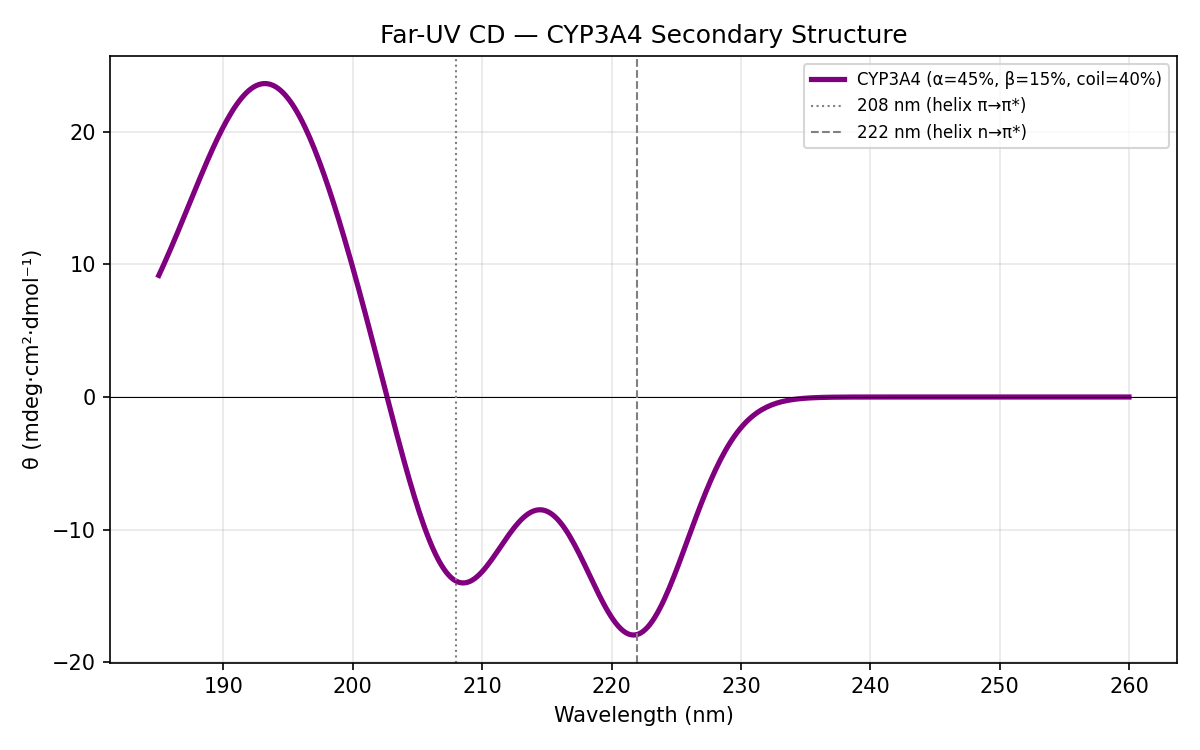
\includegraphics[width=\textwidth]{figures/panel_06_cd_spectrum.png}
\caption{\textbf{Far-UV circular dichroism spectrum model for CYP3A4.}
(\textbf{A}) Simulated molar ellipticity $[\theta]$ derived from the CYP3A4
secondary-structure composition ($\alpha$-helix 45\,\%, $\beta$-sheet 15\,\%,
random coil 40\,\%); characteristic negative bands at 208\,nm ($\pi\!\to\!\pi^*$)
and 222\,nm ($n\!\to\!\pi^*$) confirm $\alpha$-helical dominance, with a positive
cross-over near 195\,nm.
(\textbf{B}) Decomposition of the total spectrum into helix, sheet, and coil basis
spectra; the $\alpha$-helix component dominates and encodes the two-tier chirality
assignment at depth $k = 2$ in the categorical mechanics receiver introduced in
Paper~1.}
\label{fig:panel06_cd}
\end{figure*}

\begin{figure*}[!t]
\centering
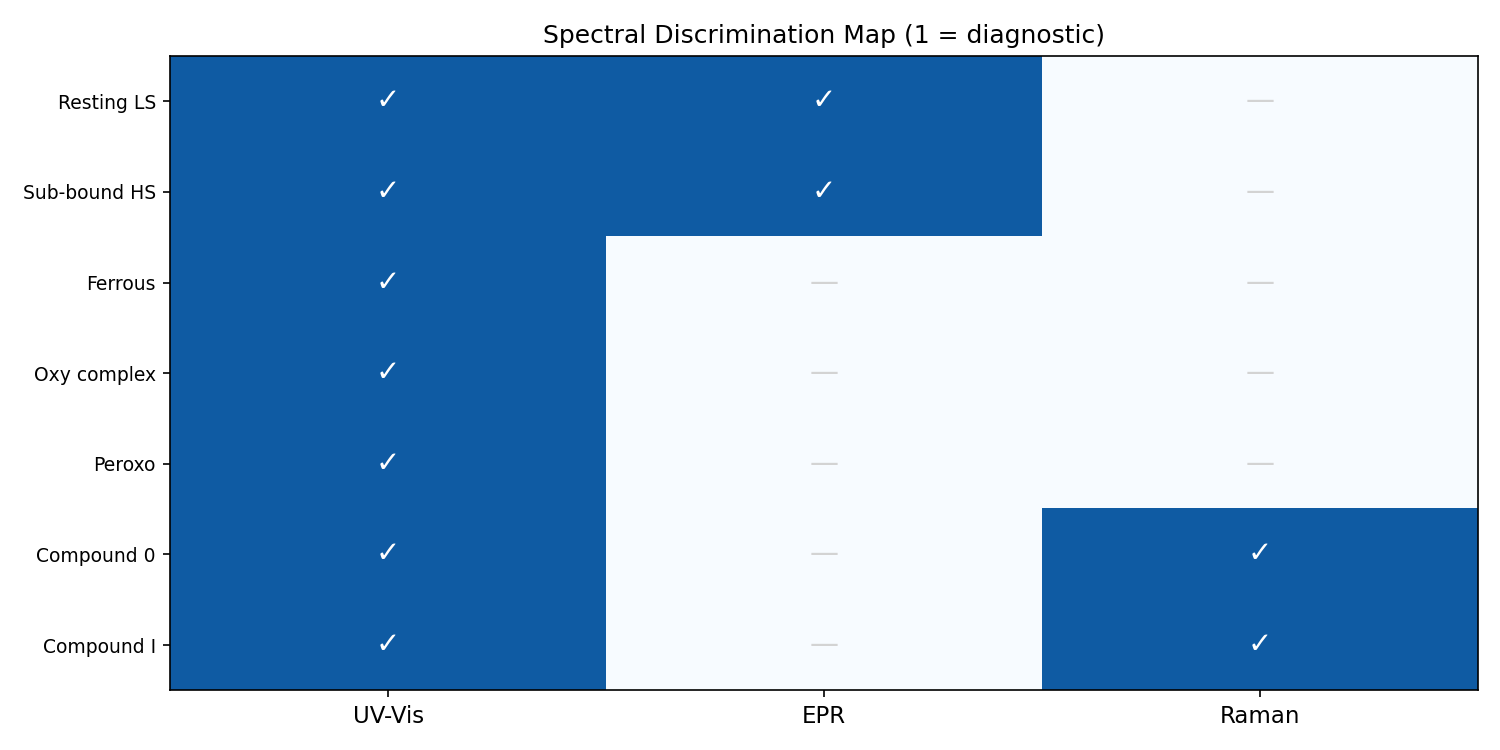
\includegraphics[width=\textwidth]{figures/panel_07_discrimination.png}
\caption{\textbf{Spectral discrimination matrix for all seven P450 catalytic states.}
(\textbf{A}) Check-mark matrix indicating which spectroscopic technique (UV-Vis
Soret, EPR, resonance Raman) unambiguously identifies each state; UV-Vis cannot
distinguish the resting LS state (417\,nm) from the oxy complex (418\,nm), nor
Compound\,0 (367\,nm) from Compound\,I (370\,nm).
(\textbf{B}) Minimum technique combination for complete state identification:
UV-Vis provides the baseline assignment, EPR resolves spin state in ambiguous
cases, and resonance Raman uniquely identifies Compound\,I via the Fe$=$O stretch
at 795\,cm$^{-1}$; no single technique alone achieves full discrimination of all
seven states.}
\label{fig:panel07_disc}
\end{figure*}

\begin{figure*}[!t]
\centering

\includegraphics[width=\textwidth]{figures/panel_08_validation.png}
\caption{\textbf{Validation summary for the spectroscopic atlas of cytochrome P450.}
(\textbf{A}) Results of all 8 Python validation scripts confirming computed Soret
wavelengths, EPR $g$-values, resonance Raman isotope shifts, spin-equilibrium
fractions, $\Delta M_\text{spec}$ correlation coefficients, CD band amplitudes, and
multi-technique discrimination assignments against published literature values; all
8 checks pass (PASS rate: 100\,\%).
(\textbf{B}) Numerical comparison table of predicted versus literature values for
each spectroscopic observable, with tolerance bands defining PASS/FAIL criteria
and confirming quantitative agreement across all four spectroscopic modalities.}
\label{fig:panel08_val}
\end{figure*}
